\documentclass[margin=3mm]{standalone}
\usepackage{tikz}
\usetikzlibrary{shapes.geometric, arrows}

\tikzstyle{startstop} = [rectangle, rounded corners, minimum width=2cm, minimum height=1cm, text centered, draw=black, text=white, fill=black!80]
\tikzstyle{statement} = [rectangle, minimum width=4cm, minimum height=1cm, text centered, draw=black, fill=blue!20]
\tikzstyle{decision} = [rectangle, minimum height=1cm, text centered, draw=black, fill=yellow!30]
\tikzstyle{edge} = [thick, ->, >=stealth]

\begin{document}
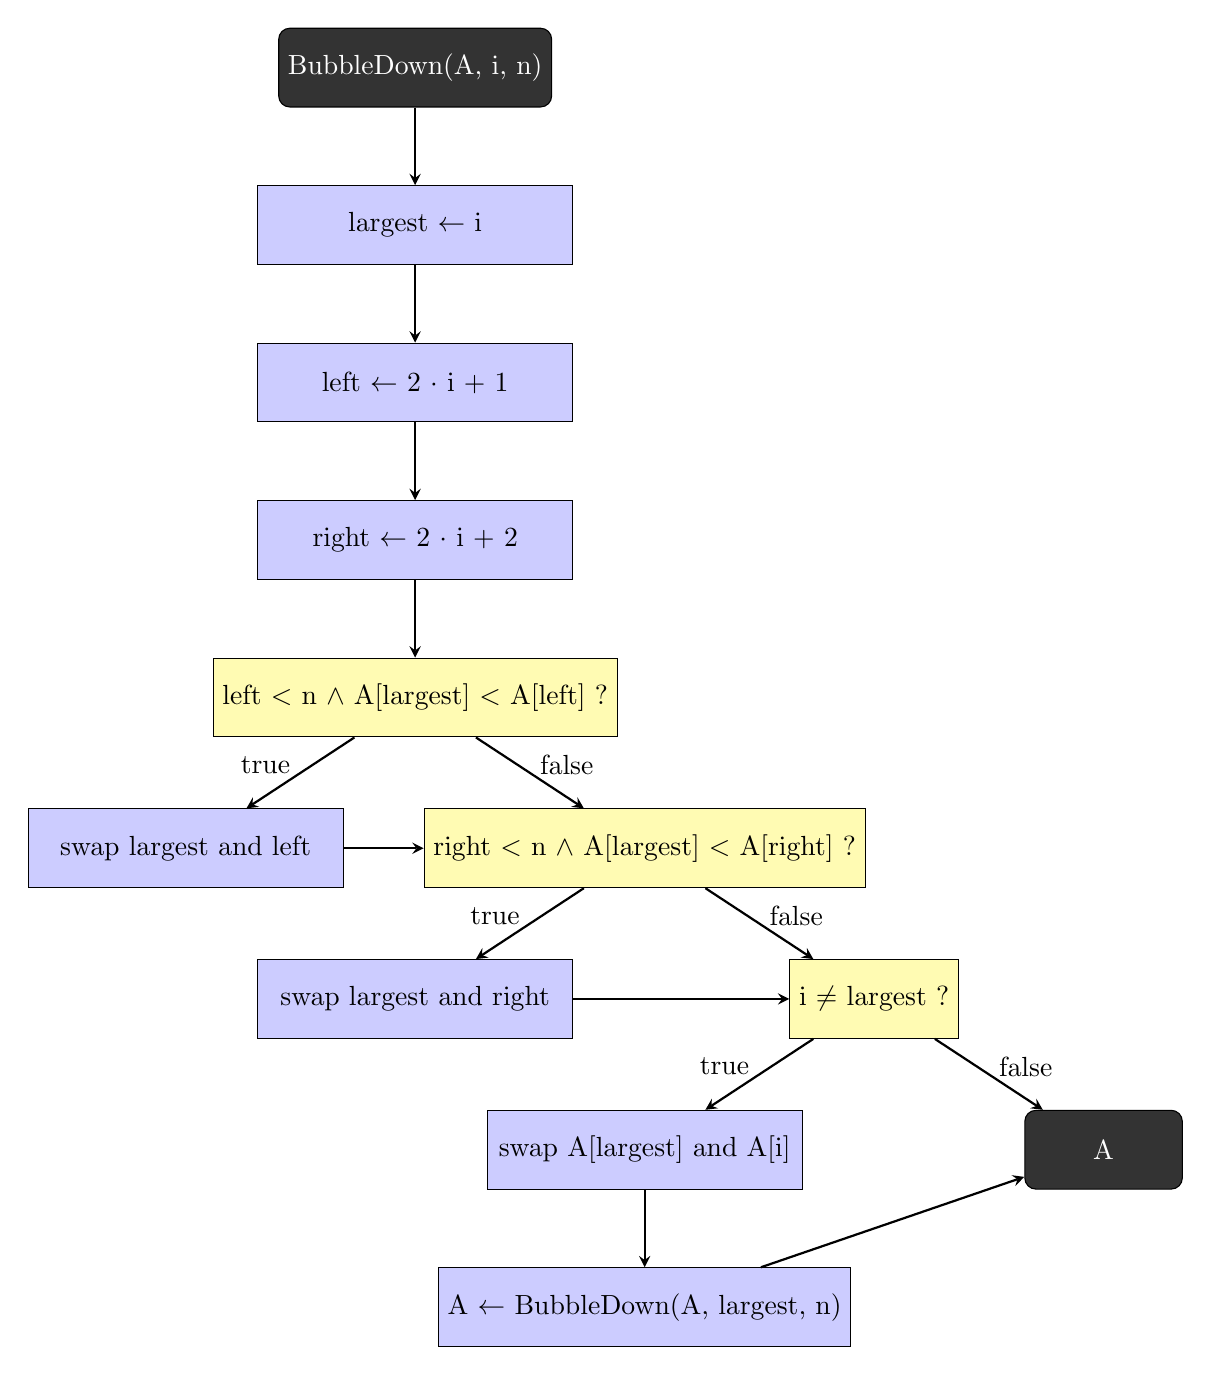
\begin{tikzpicture}[node distance=2cm]

\node (0) [startstop] {BubbleDown(A, i, n)};
\node (1) [statement, below of=0] {largest $\gets$ i};
\node (2) [statement, below of=1] {left $\gets$ 2 $\cdot$ i + 1};
\node (3) [statement, below of=2] {right $\gets$ 2 $\cdot$ i + 2};
\node (4) [decision, below of=3] {left $<$ n $\land$ A[largest] $<$ A[left] ?};
\node (5) [statement, yshift=-0.5cm, xshift=-1.5cm, below left of=4] {swap largest and left};
\node (6) [decision, yshift=-0.5cm, xshift=1.5cm, below right of=4] {right $<$ n $\land$ A[largest] $<$ A[right] ?};
\node (7) [statement, yshift=-0.5cm, xshift=-1.5cm, below left of=6] {swap largest and right};
\node (8) [decision, yshift=-0.5cm, xshift=1.5cm, below right of=6] {i $\neq$ largest ?};
\node (9) [statement, yshift=-0.5cm, xshift=-1.5cm, below left of=8] {swap A[largest] and A[i]};
\node (10) [statement, below of=9] {A $\gets$ BubbleDown(A, largest, n)};
\node (11) [startstop, yshift=-0.5cm, xshift=1.5cm, below right of=8] {A};

\draw [edge] (0) -- (1);
\draw [edge] (1) -- (2);
\draw [edge] (2) -- (3);
\draw [edge] (3) -- (4);
\draw [edge] (4) -- node[anchor=west, yshift=0.1cm]{false} (6);
\draw [edge] (4) -- node[anchor=east, yshift=0.1cm]{true} (5);
\draw [edge] (5) -- (6);
\draw [edge] (6) -- node[anchor=west, yshift=0.1cm]{false} (8);
\draw [edge] (6) -- node[anchor=east, yshift=0.1cm]{true} (7);
\draw [edge] (7) -- (8);
\draw [edge] (8) -- node[anchor=west, yshift=0.1cm]{false} (11);
\draw [edge] (8) -- node[anchor=east, yshift=0.1cm]{true} (9);
\draw [edge] (9) -- (10);
\draw [edge] (10) -- (11);

\end{tikzpicture}
\end{document}